\documentclass[a4paper,openright,12pt, oneside]{book}
\usepackage[spanish]{babel} 
\usepackage[latin1]{inputenc}
\usepackage{url}
\usepackage{graphics,graphicx}
\usepackage{algpseudocode}
\usepackage{colortbl}
\usepackage{anysize} %Para los margeness
\usepackage{array}
\usepackage{multirow} % para unir filas
\usepackage{multicol}
\usepackage{dsfont}
\usepackage{blkarray}
\usepackage{amsmath} %para hacer la combinatoria
\usepackage{listings}
\usepackage{mathtools}
\usepackage{tabularx,ragged2e}
\usepackage{titlesec}
\graphicspath{ {img/} }
\usepackage[]{algorithm2e}
\lstset{ %
language=Php,                % choose the language of the code
basicstyle=\footnotesize,       % the size of the fonts that are used for the code
numbers=left,                   % where to put the line-numbers
numberstyle=\footnotesize,      % the size of the fonts that are used for the line-numbers
stepnumber=1,                   % the step between two line-numbers. If it is 1 each line will be numbered
numbersep=5pt,                  % how far the line-numbers are from the code
backgroundcolor=\color{white},  % choose the background color. You must add \usepackage{color}
showspaces=false,               % show spaces adding particular underscores
showstringspaces=false,         % underline spaces within strings
showtabs=false,                 % show tabs within strings adding particular underscores
frame=single,           % adds a frame around the code
tabsize=2,          % sets default tabsize to 2 spaces
captionpos=b,           % sets the caption-position to bottom
breaklines=true,        % sets automatic line breaking
breakatwhitespace=false,    % sets if automatic breaks should only happen at whitespace
mathescape=true, %para agregar simbolos YOOOOO
escapeinside={\%*}{*)}          % if you want to add a comment within your code
}

\DeclarePairedDelimiter\norm{\lVert}{\rVert}
\DeclareRobustCommand{\orderof}{\ensuremath{\mathcal{O}}}
\DeclareRobustCommand{\matrix}{\ensuremath{\mathcal{M}}}
\newcommand{\sii}{\Leftrightarrow}
\newcommand{\reales}{\mathds{R}}
\newcommand{\enteros}{\mathds{Z}}
\newcommand{\nat}{\mathds{N}}
\newcommand{\infinito}{\infty}
\def\blacksquare{\hbox{\vrule width 5pt height 5pt depth 0pt}}
\def\fin{\ \ \ \hbox{}\nolinebreak\hfill $\blacksquare \  \  \  \  $ \par{}\medskip}

\newcommand{\implica}{\rightarrow}



\makeatletter
\newif\if@borderstar
\def\bordermatrix{\@ifnextchar*{%
\@borderstartrue\@bordermatrix@i}{\@borderstarfalse\@bordermatrix@i*}%
}
\def\@bordermatrix@i*{\@ifnextchar[{\@bordermatrix@ii}{\@bordermatrix@ii[()]}}
\def\@bordermatrix@ii[#1]#2{%
\begingroup
\m@th\@tempdima8.75\p@\setbox\z@\vbox{%
\def\cr{\crcr\noalign{\kern 2\p@\global\let\cr\endline }}%
\ialign {$##$\hfil\kern 2\p@\kern\@tempdima & \thinspace %
\hfil $##$\hfil && \quad\hfil $##$\hfil\crcr\omit\strut %
\hfil\crcr\noalign{\kern -\baselineskip}#2\crcr\omit %
\strut\cr}}%
\setbox\tw@\vbox{\unvcopy\z@\global\setbox\@ne\lastbox}%
\setbox\tw@\hbox{\unhbox\@ne\unskip\global\setbox\@ne\lastbox}%
\setbox\tw@\hbox{%
$\kern\wd\@ne\kern -\@tempdima\left\@firstoftwo#1%
\if@borderstar\kern2pt\else\kern -\wd\@ne\fi%
\global\setbox\@ne\vbox{\box\@ne\if@borderstar\else\kern 2\p@\fi}%
\vcenter{\if@borderstar\else\kern -\ht\@ne\fi%
\unvbox\z@\kern-\if@borderstar2\fi\baselineskip}%
\if@borderstar\kern-2\@tempdima\kern2\p@\else\,\fi\right\@secondoftwo#1 $%
}\null \;\vbox{\kern\ht\@ne\box\tw@}%
\endgroup}

\begin{document}

\begin{titlepage}

\begin{center}
\vspace*{-1in}


FACULTAD DE MATEM\'ATICA, ASTRONOM\'IA, F\'ISICA Y COMPUTACI\'ION\\
\vspace*{0.15in}
DEPARTAMENTO DE COMPUTACI\'ON \\
\vspace*{0.6in}
\begin{large}
\end{large}
\vspace*{0.2in}
\begin{Large}
\textbf{TITULO} \\
\end{Large}
\vspace*{0.3in}
\begin{large}
Tesis realizada por Emanuel Emilio Lupi para la Licenciatura en Ciencias de la Computaci\'on en la Universidad Nacional de C\'ordoba\end{large}

\vspace*{0.3in}
\rule{80mm}{0.1mm}\\
\vspace*{0.1in}
\begin{large}
Dirigida por: \\
Doctor\\
Doctor\\
\vspace*{0.1in}
\end{large}
\end{center}
\end{titlepage}

\mbox{}
\thispagestyle{empty}
\pagenumbering{arabic}

\chapter*{Agradecimientos} % si no queremos que a\~nada la palabra "Capitulo"
\addcontentsline{toc}{chapter}{Agradecimientos} % si queremos que aparezca en el \'indice
\markboth{AGRADECIMIENTOS}{AGRADECIMIENTOS} % encabezado

\begin{itemize}
\item A mi familia, quienes siempre ser\'an los primeros agradecidos en
cualquier logro de mi vida por formarme como persona, por el amor y el apoyo incondicional que siempre me brindan.

\item A mis directores Nicolas y Mariano por la calidez humana y la gran ayuda que siempre me prestaron a lo largo del proyecto.

\item A mis amigos y compa\~neros Kevin, Fernando, Franco, Emiliano, Maxi, Eric, H\'ector, Elias, Pablo, Ezequiel, Agustin, Leandro, Emanuel, Joaquin, Fede, Gonza, Alan, Agus, Demetrio y tantos mas.

\item Al Ingeniero Marcelo Cometto por darme la posibilidad de crecer profesionalmente y confiar en mi.
\end{itemize}

\chapter*{\hspace{0.65cm}Resumen} % si no queremos que a\~nada la palabra "Capitulo"
\addcontentsline{toc}{chapter}{Resumen} % si queremos que aparezca en el \'indice
\markboth{RESUMEN}{RESUMEN} % encabezado

El problema consiste en resolver la ecuaci\'on de Schrodinger independiente del tiempo, usando el conjunto de funciones conocido como B-splines.

La ecuaci\'on de Schr\"odinger independiente del tiempo predice que las funciones de onda pueden tener la forma de ondas estacionarias, denominados estados estacionarios (tambi\'en llamados ``orbitales``, como en los orbitales at\'omicos o los orbitales moleculares). Estos estados son importantes, y si los estados estacionarios se clasifican y se pueden comprender, entonces es m\'as f\'acil de resolver la ecuaci\'on de Schr\"odinger dependiente del tiempo para cualquier estado. La ecuaci\'on de Schr\"odinger independiente del tiempo es la ecuaci\'on que describe los estados estacionarios.

La ecuaci\'on de Schrodinger es una ecuaci\'on diferencial con autovalores y 
autovectores o autofunciones, las autofunciones representan los autoestados cu\'anticos del sistema 
(cuando hablamos de ecuaci\'on de Schrodinger es siempre hablando en el contexto de mec\'anica cu\'antica) y 
los autovalores asociados a cada autofuncion representa la energ\'ia de esa autofuncion.

Ahora bien, desde un punto de vista mas matem\'atico, tenemos que resolver una ecuaci\'on diferencial 
en derivadas parciales de segundo orden y desgraciadamente no existe una forma general para 
las soluciones de una ecuaci\'on diferencial arbitraria de segundo orden, por lo que hay que buscar formas 
alternativas para encontrar las soluciones o aproximaciones a las soluciones, un m\'etodo bastante 
usado, que en particular es el m\'etodo que estamos usando, se llama m\'etodo variacional de 
Rayleigh-Ritz, el cual permite resolver o encontrar las soluciones a ecs diferenciales con una alta 
precisi\'on. 

En este trabajo se recibio una implementacion \cite{HE_EFERICO} del m\'etodo variacional de Rayleigh-Ritz el cual se optimiz\'o utilizando estructuras de datos y modificaciones algoritmicas m\'as eficientes.

\tableofcontents % indice de contenidos

\setcounter{chapter}{1}
\chapter*{Introduccion}\label{Introduccion}
\addcontentsline{toc}{chapter}{Introduccion} % si queremos que aparezca en el 
\markboth{}{} % encabezado

Para el desarrollo del trabajo que presentamos en este informe, es necesario estudiar y comprender varias herramientas y t\'ecnicas que usaremos a lo largo del proyecto. A continuaci\'on presentamos un resumen de los temas que abordaremos.

\section{Motivaci\'on}

La aplicaci\'on del m\'etodo es pr\'acticamente cualquier problema de mec\'anica cu\'antica en el 
cual no se pueda encontrar una soluci\'on anal\'itica.
En la gran mayor\'ia de los problemas, no es posible encontrar una soluci\'on anal\'itica a la ecuaci\'on de Schrodinger por lo que se buscan soluciones aproximadas en forma num\'erica.

En un gran n\'umero de problemas, para obtener una buena aproximaci\'on de la soluci\'on real es necesario recurrir a tama\~nos de matrices grandes por lo que el c\'omputo y memoria de las mismas se hace cada vez m\'as lento y pesado, y es de suma importancia tener un software lo m\'as eficiente posible para dicho c\'alculo. 

\section{Objetivos del trabajo}

El objetivo del trabajo es mejorar una implementaci\'on existente de del m\'etodo variacional de Rayleigh-Ritz en cuanto a eficiencia de tiempo y memoria del calculo a travez de estructuras de datos especificas (como son matrices dispersas) y utilizando arquitecturas de GPU en algunas rutinas.


\section{Estructura de la Tesis}

La t\'esis esta estructurada de la siguiente manera:

\begin{itemize}
    \item Nociones Preliminares: Se introducen las estucturas de datos a utilizar, ventajas y desventajas de las mismas
    \item Modelo Computacional SIMD: Se explican los conceptos de las arquitecturas GPGPU y las t\'ecnicas de programaci\'on para su mejor desempe\~nio.
    \item Optimizaci\'on: Se desarrollan variaciones estructurales y algoritmicas. 
    \item Resultados: Se presentan los resultados obtenidos por las modificaciones.
    \item Concluciones: Se prensentan concluciones del trabajo y futuras posibles mejoras
\end{itemize}

\setcounter{chapter}{2}
\setcounter{section}{0}
\chapter*{Nociones preliminares}\label{Nociones preliminares}
\addcontentsline{toc}{chapter}{Nociones preliminares} % si queremos que aparezca en el 
\markboth{}{} % encabezado

\section{Estructura de representacion de matrices dispersas}

En esta secci\'on explicaremos las estructuras de representaciones de matrices.

A medida que el problema crece las matrices se vuelven mas garndes y al mismo tiempo mas dispersas (para este problema en particular).
Un sistema linear grande de la forma $\mathcal{A}x = b$ puede ser mas eficientemente resuelto si los elementos que son ceros de $\mathcal{A}$ no son guardados. Los esquemas de almacenamiento dispersos asignan almacenamiento contiguo en memoria para los elementos distintos de cero de la matriz y tal vez un n\'umero limitado de ceros. Esto, por supuesto, requiere un esquema para saber d\'onde encajan los elementos en la matriz completa

Hay muchos m\'etodos para almacenar los datos (v\'ease por ejemplo Saad \cite{SPARSKIT} y Eijkhout \cite{LAPACK}). Aqu\'i discutiremos \textit{almacenamiento de filas y columnas comprimidas}, \textit{almacenamiento de filas comprimidas en bloques}, \textit{almacenamiento en diagonal} y \textit{almacenamiento diagonal recortado}

\subsection{Almacenamiento de filas y columnas comprimidas}

Los formatos Compressed Row y Column Storage son los m\'as generales: no hacen absolutamente ninguna suposici\'on sobre la estructura de dispersi\'on de la matriz y no almacenan elementos innecesarios. Por otra parte, no son muy eficientes, necesitando un paso de direccionamiento indirecto para cada operaci\'on escalar individual en un producto vectorial matricial o soluci\'on precondicionadora.

Este formato pone los elementos no ceros de las filas en memoria contigua. Suponiendo que tenemos una matriz dispersa no sim\'etrica $\mathcal{A}$, creamos 3 arreglos: uno con tipo float (\textit{val}), y otros dos con tipo interos (\textit{col\_ind, row\_ptr}). El arreglo \textit{val} guarda los valores de los elementos no ceros de la matriz $\mathcal{A}$. El arreglo \textit{col\_ind} guarda los indices de la columna de los elementos en el arreglo \textit{val}. Esto es: 
$$val_{k} = \mathcal{A}_{i,j} \implica col\_ind_{k} = j $$
El arreglo \textit{row\_ptr} guarda la ubicaci\'on de \textit{val} donde empieza la fila. esto es:
$$val_{k} = \mathcal{A}_{i,j} \implica row\_ptr_{i} \leq k < row\_ptr_{i+1} $$
Por convenci\'on definimos $row\_ptr_{n+1} = nnz + 1$ Donde nnz es la cantidad de numeros no ceros de la matriz $\mathcal{A}$. La memoria necesaria para este enfoque es \orderof(nnz + n)

Ejemplo: considere la siguiente matriz:

\begin{equation}
\mathcal{A} =
\left(
\begin{array}{cccccc}
 
10& 0& 0& 0& -2& 0 \\

3& 9& 0& 0& 0& 3 \\
   
0& 7& 8& 7& 0& 0 \\

3& 0& 8& 7& 5& 0 \\
   
0& 8& 0& 9& 9& 13 \\
    
0& 4& 0& 0& 2& -1 \\
\end{array}
\right)
\end{equation}

En formato CRS tendria esta forma
\begin{equation}
val = 
\left(
\begin{array}{ccccccccccccccccccc}
10& -2& 3& 9& 3 & 7& 8& 7& 3& 8& 7& 5& 8& 9& 9& 13 & 4& 2& -1 
\end{array}
\right)
\end{equation}

\begin{equation}
col\_ind = 
\left(
\begin{array}{ccccccccccccccccccc}
0 & 4 & 0 & 1 & 5 & 1 & 2 & 3 & 0 & 2 & 3 & 4 & 1 & 3 & 4 & 5 & 1 & 4 & 5
\end{array}
\right)
\end{equation}


\begin{equation}
row\_ptr = 
\left(
\begin{array}{ccccccc}
1 & 3 & 6 & 9 & 13 & 17 & 20
\end{array}
\right)
\end{equation}




El almacenamiento de columnas comprimidas es an\'alogo

\subsection{Almacenamiento de filas comprimidas en bloques.}

Si la matriz escasa se compone de bloques densos cuadrados de nonzeros en alg\'un patr\'on regular, podemos modificar el formato CRS (o CCS) para explotar tales patrones de bloque. Las matrices de bloque t\'ipicamente surgen de la discretizaci\'on de ecuaciones diferenciales parciales en las que hay varios grados de libertad asociados con un punto. Luego, la partici\'on de la matriz en bloques peque\~nos con un tama\~no igual al n\'umero de grados de libertad, y tratar cada bloque como una matriz densa, a pesar de que puede tener algunos ceros.

Sea \textit{$n_{b}$} es la dimensi\'on de cada bloque y \textit{nnzb} la cantidad de no ceros de cada bloque en la matriz $\mathcal{A}^{n,m}$, la cantidad de memoria es $\orderof(nnz)$.

\subsection{Almacenamiento en diagonal.}

Si la matriz $\mathcal{A}$ es una matriz de banda donde el ancho de la banda es susficientemente constante de fila en fila. Entonces podemos aprovechar esta estructura en el esquema de almacenamiento almacenando subdiagonales de la matriz en ubicaciones consecutivas. No s\'olo podemos eliminar el vector que identifica la columna y la fila (si lo miramos como un CRS), podemos empaquetar los elementos no nulos de tal manera que el producto vectorial sea m\'as eficiente. Este esquema de almacenamiento es particularmente \'util si la matriz surge de una discretizaci\'on de elementos finitos o diferencias finitas en una matriz de producto tensor.

Decimos que la matriz $\mathcal{A}^{m,n}$ es de banda si hay enteros no negativos \textit{p},\textit{q} tal que $\mathcal{A}_{i,j}$ $\neq$ 0 $\implica$ i-p $\leq$ j $\leq$ i + q. En este caso podemos alojar la matriz $\mathcal{A}$ en un arreglo \textit{val}(1:n, -p:q) la declaraci\'on con dimensiones invertidas corresponde a \textit{LINPACK band format} \cite{LINPACK}

Por lo general, los formatos de banda incluyen almacenar algunos ceros. El formato CDS puede incluso contener algunos elementos de matriz que no corresponden a elementos de matriz en absoluto. Consideremos la matriz no sim\'etrica definida por:

\begin{equation}
\mathcal{A} =
\left(
\begin{array}{cccccc}
 
10& -3& 0& 0& 0& 0\\
3&   9& 6& 0& 0& 0 \\
0&   7& 8& 7& 0& 0 \\
0&   0& 8& 7& 5& 0 \\
0&   0& 0& 9& 9& 13 \\
0&   0& 0& 0& 2& -1 \\
\end{array}
\right)
\end{equation}

Usando el formato CDS, alojamos la matriz $\mathcal{A}$ en un arreglo \textit{$cdsA^{6, 3}$} donde las columnas estan indexadas desde -1 usando el mapeo $val_{i, j}$ = $a_{i, i+j}$

\begin{tabular}{ l || c | c | c | c | c | c}
  val(:, -1) & 0 & 3 & 7 & 8 & 9 & 2 \\
  val(:, 0) & 10 & 9 & 8 & 7 & 9 & -1 \\
  val(:, 1) & -3 & 6 & 7 & 5 & 13 & 0 \\
\end{tabular}

Notar que los dos ceros no corresponden a un elemento existente de la matriz.

Una generalizaci\'on del formato CDS m\'as adecuada para manipular matrices dispersas generales en superordenadores vectoriales es discutido por Melhem en \cite{MELHEM}. Esta variante de CDS utiliza una estructura de datos de banda para almacenar la matriz. Esta estructura es m\'as eficiente en el almacenamiento en el caso de variar el ancho de banda, pero hace que el producto de vector de matriz sea ligeramente m\'as caro, ya que implica una operaci\'on de recopilaci\'on.

Como es definido en \cite{MELHEM}, una linea en $\mathcal{A}^{n,m}$ es un conjunto de posiciones 
S = $\{(i, \theta(i)): i \in I \subseteq I_{n} \}$ donde $I_{n}$ = ${1, ..., n}$ y $\theta$ es una funci\'on estrictamente creciente. Especificamente: 


$$(i, \theta(i)), (j, \theta(j)) \in S \implica (i < j \implica \theta(i) < \theta(j)) $$

Cuando se computa el producto Matriz-vector $ y = \mathcal{A}x $ usando rayas, cada (i, $\theta_{k}(i)$) de $\mathcal{A}$ se multiplica por $x_{\theta_{k}(i)}$ y es acumulado en $y_{i}$.


\subsection{Almacenamiento diagonal recortado.}

El formato JDS (sus siglas en ingles de Jagged Diagonal Storage) puede ser \'util para la implementaci\'on de m\'etodos iterativos en procesadores paralelos y vectoriales (v\'ease Saad \cite{JDS}). Al igual que el formato Diagonal Comprimido, da una longitud de vector esencialmente del tama\~no de la matriz. Es m\'as eficiente en cuanto a espacio que CDS a costa de una operaci\'on de recopilaci\'on / dispersi\'on.

Una forma simplificada de JDS, llamada almacenamiento de ITPACK o almacenamiento Purdue, se puede describir como sigue:

\begin{equation}
\left(
\begin{array}{cccccc}
 
10& -3& 0& 1& 0& 0\\
0&   9& 6& 0& -2& 0 \\
3&   0& 8& 7& 0& 0 \\
0&   6& 0& 7& 5& 0 \\
0&   0& 0& 0& 9& 13 \\
0&   0& 0& 0& 5& -1 \\
\end{array}
\right)
\implica
\left(
\begin{array}{cccccc}
 
10& -3& 1&  &  & \\
9& 6& -2& &  & \\
3& 8& 7& &  & \\
6& 7& 5& &  & \\
9& 13 & &  & \\
5& -1 & &  &\\
\end{array}
\right)
\end{equation}

Luego las columnas se almacenan consecutivamente. Todas las filas se rellenan con ceros a la derecha para darles la misma longitud. Correspondiente al arreglo de elementos de matriz \textit{val}(:, :), un arreglo de \'indices de columna, col\_ind (:, :) tambi\'en se almacena:

Est\'a claro que los ceros de relleno en esta estructura pueden ser una desventaja, especialmente si el ancho de banda de la matriz var\'ia fuertemente. Por lo tanto, en el formato CRS, reordenamos las filas de la matriz de forma decreciente de acuerdo con el n\'umero de elementos no ceros de una fila. Las diagonales comprimidas y permutadas se almacenan entonces en una matriz lineal. La nueva estructura de datos se denomina diagonales dentadas.



\begin{table}[htdp]
    \caption{}
    \begin{tabular}{ | l || c | c | c | c | c | c |}
      \hline
      val(:, 1) & 10 & 9 & 3 & 6 & 9 & 5 \\ \hline 
      val(:, 2) & -3 & 6 & 8 & 7 & 13 & -1 \\ \hline
      val(:, 3) & 1 & -2 & 7 & 5 & 0 & 0 \\ \hline
      val(:, 4) & 0 & 0 & 0 & 4 & 0 & 0 \\ \hline 
    \end{tabular}
\end{table}

\begin{table}[htdp]
    \caption{}
    \begin{tabular}{| l || c | c | c | c | c | c |}
        \hline
      col\_ind(:, 1) & 1 & 2 & 1 & 2 & 5 & 5 \\ \hline
      col\_ind(:, 2) & 2 & 3 & 3 & 4 & 6 & 6 \\ \hline
      col\_ind(:, 3) & 4 & 5 & 4 & 5 & 0 & 0 \\ \hline
      col\_ind(:, 4) & 0 & 0 & 0 & 6 & 0 & 0 \\ \hline
    \end{tabular}
\end{table}


El n\'umero de diagonales irregulares es igual al n\'umero de no ceros en la primera fila, es decir, el mayor n\'umero de no ceros en cualquier fila de $\mathcal{A}$. La estructura de datos para representar la matriz por lo tanto consiste en un arreglo de permutaci\'on (\textit{perm} (1: n)) que reordena las filas, un arreglo de punto flotante (jdiag (:)) que contiene las diagonales dentadas en sucesi\'on, un arreglo de enteros (\textit{col\_ind} :)) que contiene los \'indices de columna correspondientes, y finalmente un arreglo de punteros (\textit{jd\_ptr} (:)) cuyos elementos apuntan al comienzo de cada diagonal dentada. Las ventajas de JDS para las multiplicaciones matriciales son discutidas por Saad en \cite{JDS}.

El formato JDS para la matriz anterior en el uso de los arreglos lineales {perm, jdiag, col\_ind, jd\_ptr} se da a continuaci\'on (diagonales irregulares est\'an separados por punto y coma).

\begin{table}[htdp]
    \caption{}
    \begin{tabular}{ | l || c | c | c | c | c | c | c | c | c | c | c | c | c | c | c | c | c |}
        \hline
      jdiag & 6 & 9 & 3 & 10 & 9 & 5; & 7 & 6 & 8 & -3 & 13 & -1; & 5 & -2 & 7 & 1 & 4; \\ \hline
      col\_ind & 2 & 2 & 1 & 1 & 5 & 5; & 4 & 3 & 3 & 2 & 6 & 6; & 5 & 5 & 4 & 4 & 6; \\ \hline
    \end{tabular}
\end{table}

\begin{table}[htdp]
    \caption{}
    \begin{tabular}{ | l || c | c | c | c | c | c |}
        \hline
        perm & 4 & 2 & 3 & 1 & 5 & 6 \\ \hline
    \end{tabular}
\end{table}

\begin{table}[htdp]
    \caption{}
    \begin{tabular}{ | l || c | c | c | c | }
        \hline
      perm & 1 & 7 & 13 & 17 \\ \hline
    \end{tabular}
\end{table}



\section{Problema de autovalores y autovectores}

Como vimos anteriormente el metodo requiere que se calcule los autovalores mas peque\~nos para lograr eso se utiliz\'o paquete ARPACK.

Este paquete est\'a dise\~nado para calcular algunos autovalores y vectores propios correspondientes de una matriz general n por n A. Es m\'as apropiado para matrices grandes escasas o estructuradas A donde estructurado significa que un producto vectorial matricial w = $\mathcal{A}$*v requiere $\orderof(m)$ en lugar de $\orderof(n^{2})$ donde m es menor que n operaciones de punto flotante. Este software se basa en una variante algor\'itmica del proceso Arnoldi llamado Implicitly Restarted Arnoldi Method (IRAM). Cuando la matriz A es sim\'etrica, se reduce a una variante del proceso de Lanczos denominado M\'etodo Lanczos Impl\'icitamente Reiniciado (IRLM). Estas variantes pueden ser vistas como una s\'intesis del proceso de Arnoldi\/ Lanczos con la t\'ecnica QR impl\'icitamente desplazada que es adecuada para problemas a gran escala. Para muchos problemas est\'andar, no se requiere una factorizaci\'on de matriz. S\'olo se necesita la acci\'on de la matriz sobre un vector.

ARPACK es capaz de resolver grandes problemas simb\'olicos sim\'etricos, no sim\'etricos y generalizados de \'areas de aplicaci\'on significativas. El software est\'a dise\~nado para calcular algunos (k) valores propios con caracter\'isticas especificadas por el usuario tales como los de mayor parte real o mayor magnitud. Los requisitos de almacenamiento est\'an en el orden \orderof(n * k) de memoria. No se requiere almacenamiento auxiliar. Se calcula un conjunto de vectores de base de Schur para el eigen-espacio k-dimensional deseado que es num\'ericamente ortogonal a la precisi\'on de trabajo.

A continuaci\'on daremos una breve explicaci\'on de metodos num\'erocos utilizados para respover el problema de autovalores y autovector.

Para mas detalles ver \cite{libromagico}

\subsection{Algoritmo de Lanczos}

Este algoritmo hecho por Lanczos es un algoritmo iterativo, es una adaptacion al metodo de las potencias para calcular los autovalores y autovectores mas significativos de un sistema lineal $n^{2}$.

\subsubsection{M\'etodo Iterativo}
El m\'etodo iterativo para encontrar el mayor autovalor de una matriz $\mathcal{A}$, puede resumirse se\~nalando que si ${\displaystyle x_{0}\,}$ es un vector aleatorio y ${\displaystyle x_{n+1}=Ax_{n}\,}$
Entonces para un ${\displaystyle m\,}$ grande tal que 
$
\frac{
  \displaystyle x_{n}
} 
{
  \norm{{
    \displaystyle x_{n} 
    }}
} 
$ este pr\'oximo a un autovector.

Si ${\displaystyle A=U\operatorname {diag} (\sigma _{i})U'\,} $ es la descomposici\'on en valores propios de una matriz $\mathcal{A}$, entonces ${\displaystyle A^{n}=U\operatorname {diag} (\sigma _{i}^{n})U'}$. Para $\displaystyle n$ grande la matriz diagonal de autovalores est\'a acotada por el autovalor mas grande. Luego 
$
\frac{
  \norm{{\displaystyle x_{n+1}}}
} 
{
  \norm{{
    \displaystyle x_{n} 
    }}
} 
$ converge al valor propio mas grande y 
$
\frac{
  \displaystyle x_{n}
} 
{
  \norm{{
    \displaystyle x_{n} 
    }}
} 
$ al autovector asociado. Si el autovalor mas grande esta repetido, entonces $\displaystyle x_{n} $ converge a un vector en el subespacio generado por los autovectores asociados con esos autovalores m\'as grandes. Luego de haber encontrado el primer autovector o autovalor, uno puede restringir sucesivamente el algoritmo para el espacio nulo (nucleo) de los autovectores propios conocidos para obtener el segundo autovector o autovalor mas grande y as\'i sucesivamente.

En la pr\'actica, este sencillo algoritmo no funciona muy bien para el c\'alculo de muchos autovalores, ya que cualquier error de redondeo podr\'ia introducir ligeros cambios a los componentes de los autovectores m\'as significativos. Degradando la exactitud del c\'omputo.

\subsubsection{M\'etodo Lanczos}
Durante el procedimiento de aplicaci\'on del m\'etodo, al obtener el \'ultimo valor propio ${\displaystyle A^{n-1}v}$, tambi\'en se obtiene una serie de vectores ${\displaystyle A^{j}v,\,j=0,1,\cdots ,n-2}$ los cuales son descartados. Como ${\displaystyle n}$ es grande, puede que se tenga una gran cantidad de informaci\'on que no se utilice. Los algoritmos m\'as avanzados, Como el el algoritmo de Arnoldi, guardan esta informaci\'on y utilizan el proceso de Gram-Schmidt o el algoritmo Householder para ortogonalizar nuevamente en una base que abarca el subespacio de Krylov correspondiente a la matriz ${\displaystyle A}$.

\subsubsection{El algoritmo}

Se decea calcular la matriz tridiagonal sim\'etrica ${\displaystyle T_{mm}=V_{m}^{*}AV_{m}.} {\displaystyle T_{mm}=V_{m}^{*}AV_{m}.}$

Los elementos de la diagonal se denotan por ${\displaystyle \alpha _{j}=t_{jj}=t_{jj} }$, Y los elementos fuera de la diagonal son denotados por ${\displaystyle \beta _{j}=t_{j-1,j}}$.

\subsubsection{Iteraci\'on}

En principio, hay cuatro maneras de escribir el procedimiento de iteraci\'on.
Paige[1972] y otros trabajos muestran que el siguiente algoritmo es el m\'as estable numericamente. \cite{Cullum} \cite{booksaad}


\begin{algorithm}
    \underline{Iteraci\'on}\;
    ${v_{0}} = 0$\\

    \For{$j = 1$ to $m-1$}
    {
      $w_j = Av_j$ \\
      $\alpha_j = w_j \cdot v_j $\\
      $w_j = w_j - \alpha_j v_j - \beta_j v_{j-1}$ \\
      $\beta_{j+1} = \norm{w_j}$ \\
      $v_{j+1} = w_j / \beta_{j+1}$\\ 
    }

    $w_m = Av_m$ \\
    $\alpha_m = w_m \cdot v_m $\\
    \caption{Iteraci\'on en el algoritmo de Lanczos}

\end{algorithm}

Luego de la iteraci\'on, se obtiene $\alpha_j$ y $\beta_j$ con los que se forma la matriz tridiagonal.

\begin{equation}
\mathcal{T} =
\left(
\begin{array}{cccccc}
\alpha_1 & \beta_2& & & & 0\\
\beta_2&   \alpha_2& \beta_3& & &  \\
&   \beta_3& \alpha_3& \beta_4& &  \\
&   & \ddots& \ddots& \ddots&  \\
&   & & \beta_{m-1}& \alpha_{m-1}& \beta_{m} \\
0&   & & & \beta_{m}& \alpha_{m} \\
\end{array}
\right)
\end{equation}

Despues que la matr\'iz $\displaystyle T$ es calculada, se pueden obtener sus autovalores $\lambda_i^{(m)}$ y sus correspondientes autovectores (usando por ejemplo QR o Multiple Robust Representation MRRR).
Los autovalores pueden ser calculados en $\orderof(m^2)$ usando MRRR.
Los valores propios calculados son aproximaci\'on de los valores propios de $\displaystyle A$

\subsection{Algoritmo de Arnoldi}

El met\'odo de Arnoldi se introdujo por primera vez como un algoritmo directo para reducir una matriz general en la forma superior de Hessenberg \cite{FORMHESS}. M\'as tarde se descubri\'o que este algoritmo conduce a una buena t\'ecnica iterativa para aproximar valores propios de grandes matrices dispersas.

El algoritmo functiona para matrices no hermitaneas. Es muy \'util para casos en los que la matriz $\displaystyle A$ es grande, pero los productos de vector de matriz son relativamente baratos de realizar. Esta es la situaci\'on, por ejemplo, cuando $\displaystyle A $ es grande y escaso. Comenzamos con una presentaci\'on del agoritmo b\'asico y luego describimos una serie de variaciones.

\subsubsection{Algoritmo Basico}
El m\'etodo de Arnoldi es un m\'etodo de proyecci\'on ortogonal sobre un subspacio de Krylov. Comienza con el procedimiento de Arnoldi como se describe en el algoritmo [sitar al algoritmo]. El procedimiento puede ser visto esencialmente como un proceso de Gram-Schmidt midificado para construir una base ortogonal del subespacio de Krylov. $\displaystyle K^{m}(A,v) $


\begin{algorithm}
    \label{alg:arnoldi}
    \underline{Procedimiento Arnoldi}\;
    ${v_{1}} = v/\norm{v}_{2} $\\

    \For{$j = 1$ to $m$}
    {
      $w = Av_j$ \\
      \For{$j = 1$ to $j$}
      { 
        $h_{ij} = w*v_i$\\
        $w = w - h_{ij}v{i}$\\
      }
      $h_{j+1, k} = \norm{w}_2$\\
      \If {$h_{j+1, j}$ == $0$} {
        $stop$
       }
      
      $v_{j+1} = w/h_{j+1, j}$\\
    }
    \caption{Procedimiento de Arnoldi}

\end{algorithm}

El proceso [citar el proceso] se detendr\'a si el vector $\displaystyle w$ tiene norma 0 (desaparece).  Los vectores $ v_1, v_2, \ldots, v_m $ forman un sistema ortonormal por construcci\'on y se llaman vectores de Arnoldi. Un argumento de inducci\'on f\'acil demuestra que este sistema es una base del subespacio de Krylov $ \ KK^m(A, v) $.

A continuaci\'on se considera una relaci\'on fundamental entre las cantidades generadas por el algoritmo. La siguiente igualdad se deriva f\'acilmente:


\begin{equation}
A v_j = \sum_{i=1}^{j+1} h_{ij} v_i , \quad j=1,2,\ldots ,m \ .
\end{equation}


Si denotamos por $ V_m $ la matriz $ n \times m $ con vectores columna $ v_1,
\ldots , v_m $ y $ H_m $ la matriz $ m \times m $ Hessenberg cuyas entradas no nulas $ h_{ij} $ son definidas por el algoritmo, entonces las siguientes relaciones se mantienen:

\begin{equation}
\label{eq:AVm}
\displaystyle A V_m \textstyle = \displaystyle V_m H_m + h_{m+1,m} v_{m+1} e_m^{\ast}
\end{equation}

\begin{equation}
\label{eq:VmTAVm}
\displaystyle V_m^{\ast} A V_m \textstyle = \displaystyle H_m.
\end{equation}

La ecuaci\'on \ref{eq:VmTAVm} viene de \ref{eq:AVm} multiplicando las dos partes de la ecuacion \ref{eq:AVm} por $ V_m^{\ast}$ y usando de la ortonormalidad de $\{ v_1, \ldots,v_m \} $.

Como se observ\'o anteriormente, el algoritmo se descompone cuando la norma de $ w $  desaparece en un cierto paso $ j $. Como resulta, esto ocurre si y s\'olo si el vector de partida $ v $ es una combinaci\'on de $ j $ vectores propios (es decir, el polinomio m\'inimo de $ v_1 $ es de grado $ j $). Adem\'as, el subespacio $ \ KK_j $ es entonces invariante y los autovalores y autovectores aproximados son exactos. \cite{SaadNumMeth}

Los autovalores aproximados $ \lambda_i ^{m} $ dados por el proceso de proyecci\'on sobre $ K_m $ son los valores propios de la matriz de Hessenberg $ H_m $. Estos son conocidos como valores de Ritz. Un autovector aproximado de Ritz asociado con un valor de Ritz $ \lambda_i ^ {m} $ es definido por $ u_i ^ {m} = V_m y_i ^ {m} $, donde $
Y_i ^ {m} $ es un vector propio asociado con el autovalor $ \lambda_i ^ {m} $. Un n\'umero de los valores propios del Ritz, t\'ipicamente una peque\~na fracci\'on de $ m $, generalmente constituyen buenas aproximaciones para los valores propios correspondientes $ \lambda_i $ de $ A $, y la calidad de la aproximaci\'on usualmente mejorar\'a a medida que $ m $ aumenta.

El algoritmo original consiste en aumentar $ m $ hasta que todos los autovalores deseados de $ A $ se encuentren. Para matrices grandes, esto resulta costoso tanto en t\'erminos de c\'alculo como de almacenamiento. En t\'erminos de almacenamiento, necesitamos mantener $ m $ vectores de longitud $ n $ m\'as una matriz $ m \times m $ Hessenberg, un total de aproximadamente $ n m + m ^ 2/2 $. Para los costos aritm\'eticos, necesitamos multiplicar $ v_j $ por $ A $, al costo de $ 2 \ times N_z $, donde $ N_z $ es el n\'umero de elementos no nulos en $ A $, y luego ortogonalizar el resultado contra $ j $ Vectores al costo de $ 4 (j + 1) n, $ que aumenta con el paso n\'umero $ j $. Por lo tanto, un procedimiento de Arnoldi de $ m $ -dimensionales cuesta $ \ approx n m + m ^ 2/2 $ en almacenamiento y $ \ approx N_z + 2 n m ^ 2 $ en operaciones aritm\'eticas.


Obtener la norma residual, para un par Ritz, a medida que el algoritmo progresa es bastante eficiente. Sea $Y_y $ $ m {m} $ sea un autovector de $ H_m $ asociado al autovalor $ \lambda_i ^ {m} $, y sea $ u_i ^ {m} $ el autovector aproximado de Ritz $ u_i ^ {m} = V_m y_i ^ {m} $. Tenemos la relaci\'on.

\begin{displaymath}
(A - \lambda_i ^{m}I ) u_i ^{m}= h_{m+1,m}(e_m^{\ast} y_i^{m})v_{m+1},
\end{displaymath}

y por lo tanto,

\begin{displaymath}
\Vert ( A - \lambda_i ^{m}I ) u_i ^{m}\Vert _2 = h_{m+1,m} \vert e_m^{\ast} y_i
^{m}\vert \ .
\end{displaymath}

As\'i, la norma residual es igual al valor absoluto del \'ultimo componente del vector propio $
Y_i ^ {m} $ multiplicado por $ h_ {m + 1, m} $. Las normas residuales no son siempre indicativas de errores reales en $ \lambda_i ^ {m} $, pero pueden ser muy \'utiles para derivar procedimientos de detenci\'on.

\subsubsection{Variantes}

La descripci\'on del procedimiento de Arnoldi dado anteriormente se bas\'o en el proceso modificado de Gram-Schmidt. Otros algoritmos de ortogonalizaci\'on podr\'ian ser utilizados. Una mejora es recuperar la ortogonalidad cuando sea necesario. Cada vez que se calcula el vector final obtenido al final del segundo bucle en el algoritmo anterior, se realiza una prueba para comparar su norma con la norma del $ w $ inicial (que es $ \Vert A v_j \Vert_2 $). Si la reducci\'on cae por debajo de un determinado umbral (una indicaci\'on de que puede haber ocurrido una cancelaci\'on severa), se realiza una segunda ortogonalizaci\'on. Se sabe por un resultado de Kahan que m\'as de dos ortogonalizaciones son superfluas (v\'ease, por ejemplo, Parlett \cite{Parlett})

Una de las t\'ecnicas de ortogonalizaci\'on m\'as confiables, desde el punto de vista num\'erico, es el algoritmo Householder \cite{Householder}. Esto ha sido implementado para el procedimiento de Arnoldi por Walker \cite{Householder2}. El algoritmo Householder es num\'ericamente m\'as estable que las versiones de Gram-Schmidt o Gram-Schmidt modificado, pero tambi\'en es m\'as caro, requiriendo aproximadamente el mismo almacenamiento que el Gram-Schmidt modificado, pero aproximadamente el doble de operaciones. La ortogonalizaci\'on de Householder es una opci\'on razonable cuando se desarrollan paquetes de software confiables y de prop\'osito general donde la robustez es un criterio cr\'itico.

\subsubsection{Reinicios expl\'icitos}

Como se mencion\'o anteriormente, las implementaciones est\'andar del m\'etodo Arnoldi est\'an limitadas por sus altos requisitos de almacenamiento y computaci\'on a medida que $ m $ crece. Supongamos que estamos interesados en un solo autovalor / autovector de $ A $, llamado el autovalor de la parte real m\'as grande de $ A $. Entonces una manera de eludir la dificultad es reiniciar el algoritmo. Despu\'es de una corrida con vectores de $ m $ Arnoldi, calculamos el vector propio aproximado y lo usamos como vector inicial para la siguiente ejecuci\'on con el m\'etodo de Arnoldi. Este proceso, el m\'as simple de este tipo, es iterado a la convergencia para calcular un par propio. Para el c\'alculo de otros pares autovector autovalor, y para mejorar la eficiencia del proceso, se han desarrollado una serie de estrategias, que est\'an algo relacionadas. Estos incluyen procedimientos de deflaci\'on brevemente discutidos en la siguiente secci\'on, y la estrategia de reinicio expl\'icito descrita en \ref{alg:ERAM}

\begin{algorithm}
    \label{alg:ERAM}
    label:\\
    Iterate: Hacer m iteraciones del algoritmo \ref{alg:arnoldi}\\
    Reiniciar: Calcular el autovalor aproximado $u_1^{(m)}$ asociado con el autovalor mas a la derecha 
    $\lambda_1^{(m)}$\\
    \If {$satisface$} {
        $Stop$ \\
    }
    $v_1 = u_1^{(m)}$\\
    goto label\\
    \caption{M\'etodo expl\'icito de Arnoldi reiniciado para NHEP}
\end{algorithm}

 \subsubsection{Deflaci\'on}

 Ahora consideramos la siguiente implementaci\'on que incorpora un proceso de deflaci\'on. Hasta ahora hemos descrito algoritmos que calculan s\'olo un autopar. En caso de que se busquen varias autopar, hay dos opciones posibles.

La primera es tomar $ v_1 $ como una combinaci\'on lineal de los vectores propios aproximados cuando reiniciamos. Por ejemplo, si necesitamos calcular los vectores propios $ p $ a la derecha, podemos tomar

\begin{displaymath}\hat v_1 = \sum_{i=1}^p \rho_i \tilde u_i, \end{displaymath}

Donde los autovalores est\'an numerados en orden decreciente de sus partes reales. El vector $ v_1 $ se obtiene luego de normalizar $ \hat v_1 $. La opci\'on m\'as simple para los coeficientes $ \rho_i $ es tomar $ \rho_i = 1, i = 1, \ldots, p $. Hay varios inconvenientes a este enfoque, el m\'as importante de los cuales es que no hay manera f\'acil de elegir los coeficientes $ \rho_i $ de una manera sistem\'atica. El resultado es que para los problemas dif\'iciles, la convergencia es dif\'icil de lograr.
Una alternativa m\'as confiable es computar un autopar a la vez y usar la deflaci\'on. La matriz $ A $ puede deflactarse expl\'icitamente construyendo progresivamente los primeros $ k $ vectores de Schur. Si ya se ha calculado una base ortogonal previa $ U_ {k-1} = [u_1, \ldots, u_ {k-1}] $ del subespacio invariante, entonces para computar el valor propio $ \lambda_{k} $, Puede trabajar con la matriz
\begin{displaymath}
\tilde A = A - U_{k-1} \Sigma U_{k-1}^{\ast}, 
\end{displaymath}


En la que $\Sigma = diag(\sigma_i)$ es una matriz diagonal de desplazamientos. Los autovalores de $ \tilde A $ consisten en dos grupos. Estos valores propios asociados con los vectores de Schur $ u_1, 
\ldots, u_{k-1} $ ser\'an cambiados a $ \tilde \lambda_i = \lambda_i - \sigma_i $ y los otros no se modificar\'an. Si se buscan los valores propios con partes reales m\'as grandes, entonces los desplazamientos se seleccionan de modo que $ \lambda_k $ se convierta en el autovalor siguiente con la parte real m\'as grande de $ \tilde A $. Tambi\'en es posible desinflar simplemente proyectando los componentes asociados con el subespacio invariante cubierto por $ U_ {k-1} $; Esto conducir\'ia a operar con la matriz.

\begin{displaymath}
\tilde A = A (I - U_{k-1} U_{k-1}^{\ast}).
\end{displaymath}

Hay que tener en cuenta que si $ A U_{k-1} = U_ {k-1} R_ {k-1} $ es la descomposici\'on parcial de Schur asociada con los primeros $ k-1 $ valores de Ritz , entonces $ \tilde A = A - U_ {k-1} R_ {k-1} U_ {k-1} ^ {\ast} $. Los valores propios asociados con los vectores Schur $ u_1, \ldots, u_ {k-1} $ ahora se mover\'an a cero.

Una mejor implementaci\'on de la deflaci\'on, que encaja bien con el procedimiento de Arnoldi, es trabajar con una sola base $ v_1, v_2, \ldots, v_m $ cuyos primeros vectores son los vectores de Schur que ya han convergido. Supongamos que $ k-1 $ tales vectores han convergido y llamamos $ v_1, v_2
, \ldots, v_ {k-1} $. Luego empezamos por elegir un vector $ v_k $ que es ortogonal a $ v_1, \ldots, v_ {k-1} $ y de norma 1. Luego realizamos $ mk $ pasos de un procedimiento de Arnoldi en el que la ortogonalidad del vector $ V_j $ contra todos los $ v_i $ anteriores, incluyendo $ v_1, \ldots, v_ {k-1} $. Esto genera una base ortogonal del subespacio. 

\begin{displaymath}
\label{set:base}
{\rm span}\{ v_1,\ldots, v_{k-1} , v_k, A v_k, \ldots, A^{m-k} v_k \} \ .
\end{displaymath} 

As\'i, la dimensi\'on de este subespacio Krylov modificado es constante e igual a $ m $ en general. A continuaci\'on se presenta un esquema de este procedimiento impl\'icito de deflaci\'on combinado con el m\'etodo Arnoldi.


\begin{algorithm}
    \label{alg:ERAMDEF}
    \SetKwInOut{Input}{Input}

    \Input{
    Matriz $A$, vector inicial $v_1$, dimensi\'on del subespacio $m$ y la cantidad de autovalores $nev$ }
    $k = 1 $ \\
    \While {$k \leq nev$}{
        \For{$j = k$ to $m$}
        {
          $w = Av_j$ \\
          $calcular un conjunto de j coeficientes h_{ij} tales que w = \sum_{i=1}^j h_{ij}v_i  es ortogonal a todos los anteriores v_i, para i = 1, 2, \ldots, j$\\
          $h_{j=1, j} = \norm{w}_2$\\
          $v_{j+1} = w / h_{j+1, j}$\\
        }
        calcular el autovector aproximado de $A$ con el autovalor $\tilde\lambda_k$ y su norma residual estimada $\rho_k$\\
        Ortonormalizar este autovector sobre todos los anteriores $v_j$ para obtener un vector de Schur aproximado $\tilde u_k$ y definir $v_k = \tilde u_k$\\
        \If {$\rho_k < tol $}
        {
            $h_{ik} = v_{i}^{*}Av_{k}, i = 1, \ldots ,k$\\
            $k = k+1$\\
        }
    }
    
    \caption{M\'etodo expl\'icito de Arnoldi reiniciado con deflaci\'on para NHEP}
\end{algorithm}

Notar que en el bucle, los vectores Schur asociados con los autovalores $ \lambda_1, \ldots, \lambda_ {k-1} $ no se tocar\'an en pasos posteriores. A veces se les denomina \"vectores bloqueados\". De manera similar, la correspondiente matriz triangular superior correspondiente a estos vectores tambi\'en est\'a bloqueada.

\begin{displaymath}
\underbrace{\left[v_1, v_2, \ldots, v_{k-1}\right.}_{Bloqueados},
\underbrace{\left. v_k, v_{k+1}, \ldots v_m \right] }_{Activos}
\end{displaymath}

Cuando converge un nuevo vector de Schur, se calcula la columna $ k $ esima de $ R $ asociada con este nuevo vector de base. En los pasos siguientes, los valores propios aproximados son los valores propios de la matriz $ m \times m $ Hessenberg $ H_m $ definida en el algoritmo y cuya $ k \times k $ principal submatrix es triangular superior. Por ejemplo, cuando $ m = 6 $ y despu\'es del segundo vector de Schur, $ k = 2 $, ha convergido, la matriz $ H_m $ tendr\'a la forma

\begin{displaymath}
H_m ~ = ~
\left[ \begin{array}{cccccc}
* & * & * & * & * & * \\
 & * & * & * & * & * \\
 &  & * & * & * & * \\
 &  & * & * & * & * \\
 &  &  & * & * & * \\
 &  &  &  & * & * \\
\end{array} \right].
\end{displaymath}

En los pasos subsiguientes, s\'olo deben considerarse los valores propios no asociados con la matriz triangular superior de $ 2 \times 2 $.

Se puede demostrar que, en aritm\'etica exacta, la matriz de Hessenberg $ H_m $ en el bloque inferior $ (2 \times 2) $ es la misma matriz que se obtendr\'ia de una corrida de Arnoldi aplicada a matriz

\begin{displaymath}
\tilde A = (I-U_{k-1} U_{k-1}^{\ast} ) A.
\end{displaymath}


Por lo tanto, estamos proyectando impl\'icitamente el subespacio invariante ya calculado desde el rango de $ A $.


\subsubsection{Reiniciado Impl\'icito del Methodo de Arnoldi}

Quiz\'as el algoritmo num\'erico m\'as exitoso para calcular los autovectores y autovalores mas completo de una matriz cuadrada general $ A $ es el algoritmo QR impl\'icitamente desplazado. Una de las claves para el \'exito de este m\'etodo es su relaci\'on con la descomposici\'on de Schur.

\begin{equation}
\label{eq:AUTU}
A = U T U^{\ast}.
\end{equation}


Esta descomposici\'on bien conocida afirma que cada matriz cuadrada $ A $ es unitariamente equivalentes a una matriz triangular superior $ T $.

El algoritmo QR produce una secuencia de transformaciones unitarias de similitud que reducen iterativamente $ A $ a la forma triangular superior. En otras palabras, calcula una descomposici\'on de Schur. Una implementaci\'on pr\'actica del algoritmo QR comienza con una transformaci\'on de similitud unitaria inicial de $ A $ a la forma condensada $ V ^ {\ast} AV = H $ donde $ H $ es Hessenberg superior ( `` casi triangular superior ``) y $ V $ es unitario. Entonces se realiza la siguiente iteraci\'on.

\begin{algorithm}
    \label{alg:SHIFTMETHOD}
    \SetKwInOut{Input}{Input}

    \Input{Matriz $A$}

    $Factorizar V^{\ast} AV = H$ \\

    \While {no converge}{
        $seleccionar el desplazamiento \mu$\\
        $QR = H - \mu I$\\
        $H = Q^{\ast} H Q$\\ 
        $V = VQ$\\
    }

    \caption{M\'etodo QR Desplazado}
\end{algorithm}

En este esquema, $ Q $ es unitaria y $ R $ es triangular superior (es decir, la factorizaci\'on QR de $ H - \mu I $). Es f\'acil ver que $ H $ es unitariamente equivalente a $ A $ a lo largo de esta iteraci\'on. La iteraci\'on se contin\'ua hasta que los elementos subdiagonales de $ H $ convergen a cero, es decir, hasta que se ha obtenido (aproximadamente) una descomposici\'on de Schur.

Si $ U_k $ representa las columnas $ k $ principales de $ U $, y $ T_k $ el principio principal $ k \times k $ submatriz de $ T $ en \ref{eq:AUTU}, entonces:

\begin{displaymath}
A U_k = U_k T_k,
\end{displaymath}

Y nos referimos a esto como una descomposici\'on parcial de Schur de $ A $. Dado que hay una descomposici\'on de Schur con los autovalores de $ A $ que aparecen en la diagonal en cualquier orden, siempre hay una descomposici\'on parcial de Schur de $ A $ con los elementos diagonales de $ T_k $ que consisten en cualquier subconjunto especificado de $ k $ autovalores de $ A $. Adem\'as, $ \mbox{span} (U_k) $ es un subespacio invariante de $ A $ para estos autovalores.

\section{Descripci\'on del Algoritmo}

En esta secci\'on describiremos teoricamente el algoritmo original y en el siguiente capitulo la version optimizada del mismo.


\setcounter{chapter}{3}
\setcounter{section}{0}
\chapter*{Modelo Computacional SIMD}\label{Modelo Computacional SIMD}
\addcontentsline{toc}{chapter}{Modelo Computacional SIMD} % si queremos que aparezca en el 
\markboth{}{} % encabezado

En esta secci\'on explicaremos el uso  GPU en el \'ambito de la programaci\'on de alto desempe\~no (HPC). Diremos las razones que motivaron su uso y como fueron evolucionando las diferentes arquitecturas.


\section{Introducci\'on}

Todos usamos nuestro ordenador, pero muchas veces no somos conscientes de la tecnolog\'ia que hay en ellos. M\'aquinas incre\'ibles que nos permiten disfrutar del ocio con videojuegos de gr\'aficos muy cercanos a la realidad, mecanismos de f\'isicas que emulan rascacielos destruidos o golpes entre dos veh\'iculos que luchan en carreras fren\'eticas. Para estas tareas el trabajo del procesador gr\'afico o GPU es fundamental.

Hoy nos adentraremos en el mundo de las tarjetas gr\'aficas, de la arquitecturas de las GPU y de sus diferencias con otro procesador, el central o CPU, mucho m\'as conocido. Porque las tarjetas gr\'aficas son esenciales en la inform\'atica actual y son parte b\'asica de lo que para muchos es importante de cara al futuro: GPGPU, o el procesamiento de datos mediante GPU. Hoy nos adentramos de lleno en este tema con nuestro especial sobre procesadores gr\'aficos.


\section{La era pre-GPU}

Las cosas han cambiado mucho desde que los ordenadores dom\'esticos empezaron a implantarse en nuestros hogares, all\'a por la d\'ecada de los 80. El hardware se sustenta sobre las mismas bases de la arquitectura von Neumann, si bien \'esta ha evolucionado de forma muy notable y los sistemas actuales son ahora mucho m\'as complejos.

El tr\'io de componentes que plante\'o John von Neumann eran tres: ALU, memoria y entrada/salida, refiri\'endose a mecanismos que procesan, almacenan y reciben/envían la informaci\'on, respectivamente. Interpretando la arquitectura en un equipo actual equivaldr\'ia a tener s\'olo un procesador, un disco, un teclado y una pantalla. Evidentemente un sistema moderno est\'a formado por muchos m\'as elementos, y entre ellos la tarjeta gr\'afica se ha convertido en uno de los actuales componentes fundamentales.

\section{Los \'origenes}

En los primeros ordenadores el procesador central -- CPU, central processing unit -- era el encargado de gestionar y procesar todo tipo de informaci\'on. Desde los datos que el usuario quería operar hasta por supuesto el sistema operativo, y con \'el su interfaz.

Si bien aquellos primeros sistemas utilizaban interfaces basadas en texto, con la llegada de las primeras interfaces gráficas el nivel de exigencia creci\'o no s\'olo en el propio sistema operativo, si no tambi\'en en muchas de las aplicaciones que empezaban a surgir por la \'epoca. Programas CAD o videojuegos, por ejemplo, requer\'ian muchos m\'as recursos para funcionar correctamente.

Llegados a este punto, los dise\~nadores de sistemas se basaron en un componente que ya exist\'ia para evolucionarlo y hacerlo crecer. Los coprocesadores matem\'aticos o FPU -- floating-point unit -- eran utilizados en muchos sistemas para acelerar el procesamiento de datos. Pueden entenderse como un segundo procesador, si bien algunas de las diferencias respecto de las CPU son muy claras: no pueden tener acceso a los datos directamente (debe ser la CPU la que gestione este apartado) o ejecutan un juego de instrucciones mucho m\'as sencillo pensado para tratar datos en coma flotante.

Las exigencias continuaron creciendo, y los sistemas de la \'epoca dispon\'ian de CPU y una FPU optativa que termin\'o convirti\'endose en fundamental: los coprocesadores matem\'aticos evolucionaron hacia las GPU, al ser el componente m\'as eficiente a la hora de procesar y determinar el aspecto gr\'afico de todo tipo de software.

\section{M\'as unidades de proceso que CPU, pero m\'as sencillas: la arquitectura de las GPU}


Los coprocesadores primero y las tarjetas gr\'aficas despu\'es plantearon una arquitectura hardware muy diferente de las utilizadas en las CPU.

En una GPU tambi\'en tendremos unidades de proceso (tradicionalmente Unified Shaders o Stream Processors), memoria (que hace las veces de memoria RAM, como un sistema de almacenamiento temporal para apoyar al procesamiento de los datos) y entrada/salida. Las GPU tambi\'en tienen sus propias bibliotecas para que los desarrolladores programen el software.

Estos Unified Shaders son los que procesan la informaci\'on gr\'afica, y a priori cuantos m\'as tengamos ser\'a mejor para la capacidad de proceso de la GPU. Este factor es importante en videojuegos, pero fundamental para uno de los usos que m\'as est\'an creciendo en los \'ultimos a\~nos: GPGPU, General-purpose computing on graphics processing units.

\section{GPGPU presente}

Los sistemas crecen, pero lo hacen debido a lo que tanto los desarrolladores como los usuarios finales van exigiendo. Los videojuegos y su calidad gr\'afica son la prueba m\'as palpable de este incremento en las capacidades de proceso, pero el uso que le damos a las GPU tambi\'en ha cambiado para adaptarse a otras posibilidades.

GPGPU es el t\'ermino que se utiliza para designar las tareas de prop\'osito general, t\'ipicamente pensadas para ser procesadas en una CPU, pero que se aprovechan del potencial de la GPU para ejecutarse en ella. Dado que los procesadores gr\'aficos son mucho m\'as eficientes en cierto tipo de operaciones, los resultados se obtendr\'an m\'as r\'apidamente.

El problema de la GPGPU es precisamente que no todas las tareas tienen que ser m\'as eficientes en una GPU. \'Estas est\'an especializadas en tareas altamente paralelizables cuyos algoritmos puedan subdividirse, procesarse por separado para luego unir los subresultados y tener el resultado final.


\section{CUDA como modelos de programaci\'on escalable}

Las arquitecturas de CPU de m\'ultiples n\'ucleos y GPU significaron que los chips 
de procesadores convencionales fueran sistemas paralelos. M\'as a\'un, su paralelismo
continua escalando con la ley de Moore. El desaf\'io es lograr construir aplicaciones
que utilicen este paralelismo y que de forma transparente escalen para aprovechar
el incremento en el n\'umero de n\'ucleos. Tal como las aplicaciones de procesamiento
gr\'afico 3D escalan su paralelismo a GPU de m\'ultiples n\'ucleos.

El modelo de programaci\'on paralelo de CUDA est\'a dise\~nado para sobreponerse a este
desaf\'io mientras facilita el aprendizaje con la utilizaci\'on del est\'andar de C.

Su modelo proporciona tres tipos de abstracciones: una jerarqu\'ia de grupos de hilos (threads),
memoria compartida y barreras de sincronizaci\'on. Estas son utilizadas por el programador
a trav\'es de un n\'umero peque\~no extensiones del lenguaje C.

Estas abstracciones proveen de paralelismo de datos de grano-fino y paralelismo de
hilos, mezclado en medio de un paralelismo de datos de grano-grueso y paralelismo de tareas.
Esto lleva al usuario a dividir el problema en subproblemas que puedan ser solucionados
independientemente en paralelo por bloques de hilos, y cada problema en partes m\'as
peque\~nas que puedan ser resueltos de forma cooperativa en paralelo por todas los
hilos de un mismo bloque.

Esta descomposici\'on preserva la expresividad del lenguaje, permitiendo a los hilos
cooperar cuando solucionan cada subproblema, y al mismo tiempo permite la escalabilidad
autom\'aticamente. De este modo, cada bloque de hilos puede ser asignado a cualquiera
de los multiprocesadores disponibles en la GPU, en cualquier orden, de forma concurrente
o secuencial, permitiendo que el c\'odigo CUDA pueda ejecutarse en cualquier n\'umero
de multiprocesadores y solo el sistema de planificaci\'on debe conocer la cantidad
f\'isica de multiprocesadores, como se ilustra en la Figura 3.1.

\begin{figure}[!htbp]
  \begin{center}
    \leavevmode

    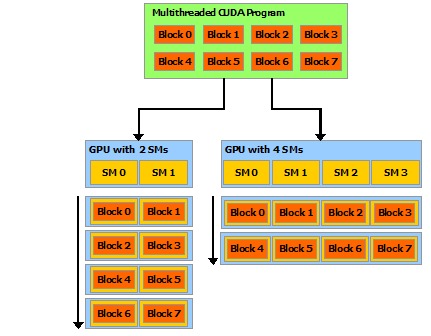
\includegraphics[]{automatic-scalability.png}

    \caption{Escalabilidad Autom\'atica}
    \label{CUDA}
  \end{center}
\end{figure}


\subsection{Modelo de programaci\'on}

En esta Secci\'on presentaremos los conceptos principales el modelo de programaci\'on
de CUDA C. CUDA C extiende el lenguaje est\'andar C, permitiendo al programador definir
funciones, llamadas \textit{Kernels}, que cuando son llamadas se ejecutan $N$ veces
en paralelo por $N$ hilos de CUDA, a diferencia de solo un hilo en una funci\'on regular
de C. El programador es qui\'en decide el valor din\'amico o est\'atico del par\'ametro $N$
en el momento de ejecutar el kernel. A cada hilo que ejecuta un kernel se le asigna
un identificador \'unico el cual es accesible por el hilo dentro del kernel. Estos identificadores
siguen los lineamientos de la jerarqu\'ia de hilos analizada a continuaci\'on.

\subsection*{Jerarqu\'ia de Hilos}

Cada identificador de hilo puede ser visto como una 3-upla, por lo que cada hilo
puede ser identificado utilizando un \'indice de una, dos o tres dimensiones. Formando as\'i
un bloque de hilos de una dos o tres dimensiones. Esto provee una forma natural de
mapear los identificadores de hilos con el accesos a datos. Hay un l\'imite en el 
n\'umero de hilos por bloques, ya que se espera que cada bloque de hilos resida en 
un mismo multiprocesador y debe compartir recursos de memoria limitados dentro
del procesador. El n\'umero m\'aximo de hilos por bloques es de 1024 en la arquitectura
utilizada en este trabajo.

Los bloques son organizados en grillas de una, dos o tres dimensiones como se ilustra
en la Figura 3.2. El n\'umero de bloques de hilos en una grilla est\'a normalmente
limitado directamente por le tama\~no de los datos a procesar o el n\'umero de procesadores
en el sistema.

\begin{figure}[!htbp]
  \begin{center}
    \leavevmode

    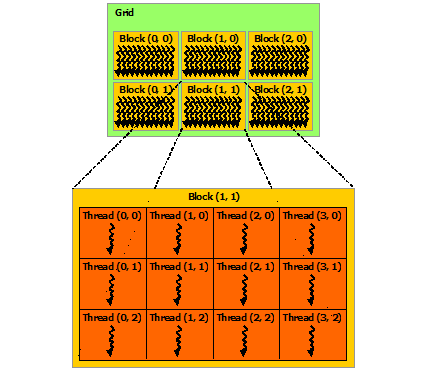
\includegraphics[]{grid-of-thread-blocks.png}

    \caption{Grilla de bloques de hilos}
    \label{CUDA}
  \end{center}
\end{figure}

Cada bloque dentro de una grilla puede ser identificado por un \'indice de una,
dos o tres dimensiones seg\'un haya sido declarado y accesible dentro del kernel
a trav\'es de una variable predefinida. Del mismo modo es accesible las dimensiones
del bloque de hilos y de la grilla de bloques. 

Los hilos dentro de un bloque pueden cooperar entre ellos compartiendo datos
a trav\'es de memoria compartida y sincronizando su ejecuci\'on para coordinar el accesos
a esta memoria. Para que la cooperaci\'on sea eficiente, se requiere que el acceso a memoria
compartida tenga baja latencia y la sincronizaci\'on no tenga una gran penalizaci\'on.

\subsection*{Jerarqu\'ia de Memoria}

Los hilos de CUDA pueden acceder a diferentes espacios de memoria durante su ejecuci\'on como
se ilustra en la Figura 3.3. Cada hilo dispone de memoria local. Cada bloque de hilos
dispone de memoria compartida visible por todos los hilos de un mismo bloque. Todos
los hilos tiene acceso a la misma memoria global.

Hay adicionalmente dos memorias de solo lectura accesible por todos los hilos: memoria
constante y memoria de textura. La memoria global, memoria de textura y memoria
constante est\'an optimizadas para diferentes usos. La memoria de textura ofrece un
modo de acceso y filtrado de datos para formatos de memoria espec\'ificos. No cubriremos
este tipo de memoria ya que no es utilizada en el trabajo.

\begin{figure}[!htbp]
  \begin{center}
    \leavevmode

    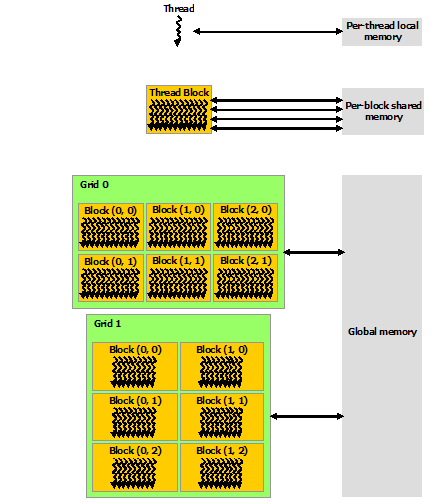
\includegraphics[]{memory-hierarchy.png}

    \caption{Jerarqu\'ia de memoria}
    \label{CUDA}
  \end{center}
\end{figure}


\subsection*{Programaci\'on Heterog\'enea}

El modelo de programaci\'on de CUDA asume que los hilos de CUDA ejecutan en un dispositivo
f\'isicamente separado que opera como un coprocesador del \textit{host} que esta ejecutando
la aplicaci\'on, por lo general y para el an\'alisis de nuestro trabajo esta aplicaci\'on 
est\'a escrita en C/C++ utilizando el lenguaje CUDA. El c\'odigo kernel ser\'a ejecutado
espec\'ificamente en la GPU y el resto del programa se ejecutar\'a en el procesador
central o CPU.

Adem\'as, el modelo computacional de CUDA asume que tanto el host como el dispositivo
manejan distintos espacios de memoria, referidos como \textit{memoria de host}
y \textit{memoria de dispositivo} respectivamente. CUDA provee una API completa
para manejar la memoria de dispositivo y poder ser alocada, escrita y le\'ida por 
el host.



\section{Implementaci\'on del hardware CUDA GPGPU}

La arquitectura de NVIDA GPU est\'a construida alrededor de un arreglo de
procesadores de flujo de m\'ultiples hilos o \textit{Streaming Multiprocessors (SMs)}.
Cuando un programa CUDA est\'a ejecutando en host e invoca la ejecuci\'on de una grilla
de kernels, los bloques de la grilla son numerados y distribuidos a los multiprocesadores
disponibles para su ejecuci\'on. Los hilos de un bloque ejecutan concurrentemente en
un mismo multiprocesador, y m\'ultiples bloques de hilos pueden ejecutar de forma
concurrente en un mismo multiprocesador. A medida que los bloques de hilos terminan,
nuevos bloques son asignados a los multiprocesadores vacantes.

Los multiprocesadores est\'an dise\~nados para ejecutar cientos de hilos de forma concurrente. 
Para manejar este n\'umero de hilos, estos utilizan una arquitectura llamada 
\textit{SIMT (Single Instruction, Multiple Thread)}


\subsection{Arquitectura SIMT}

Los multiprocesadores crean, manejan, planifican y ejecutan en paralelo grupos de 32 hilos,
llamados \textit{warps}. Cada hilo de un warp comienzan juntas en el mismo punto del
programa, pero cada uno tiene su propio contador de instrucciones y registros de estados
y son libres de ejecutar independientemente.

Cuando un multiprocesador posee uno o m\'as bloques de hilos para ejecutar, este
parte los bloques en warps y cada warp es planificada por un planificador de warps para ser ejecutada. 
La forma en que los bloques son divididos en warps es siempre la misma; cada bloque contiene
hilos con identificadores num\'ericos asignados de forma consecutiva. El primer warp contiene
los hilos con identificadores 0 a 31, la segunda warp los hilos 32 a 63 y as\'i sucesivamente.

Cada hilo dentro de una misma warp ejecuta una misma instrucci\'on al mismo tiempo, por lo tanto el rendimiento
\'optimo se consigue cuando los 32 hilos de un warp siguen el mismo camino de ejecuci\'on.
Si los hilos de un warp divergen en el flujo de ejecuci\'on, las ejecuci\'on de los 
hilos del warp son serializados, deshabilitando los hilos que no est\'an en el flujo
de ejecuci\'on y cuando los posibles caminos convergen, todos los hilos vuelven
al mismo punto del programa. Esto solo ocurre entre hilos de un mismo warp. Diferentes
warp ejecutan independientemente.

Si analizamos la correcci\'on del programa, el programador puede esencialmente
ignorar el comportamiento de la arquitectura SIMT. Sin embargo, se pueden conseguir
sustanciales resultados de mejoramiento de rendimiento teniendo en cuenta la forma
en que los hilos son agrupados y como es el comportamiento de ellos en los warps.
En la pr\'actica, esto es an\'alogo a como se comporta la cache. El tama\~no de cache
puede ser ignorado en la correcci\'on del dise\~no, pero debe ser considerado en la
estructura del c\'odigo para conseguir el rendimiento m\'aximo. La arquitectura SIMT,
requiere de ciertos cuidados al acceder a la memoria y manejar la divergencia
de los hilos, estos ser\'an analizados a m\'as adelante.

\subsection{Caracter\'isticas del Hardware Multi-hilo}

El contexto de ejecuci\'on de cada warp (contadores de programa, registros, etc.) es mantenido
en la memoria interna de cada multiprocesador lo largo de la vida del warp. Esto implica que cambiar
de un contexto de ejecuci\'on a otro no tiene costo. Esto es aprovechado para
que los multiprocesadores mantengan un conjunto de warps activas para la ejecuci\'on
y el planificador de ejecuci\'on del multiprocesador elije cual es la
siguiente warp a ejecutar. El modo de manejar la ejecuci\'on de las warps es una 
gran ventaja en el dise\~no de la arquitectura, permitiendo ocultar de forma 
\'optima la latencia de lectura y escritura a memoria, siempre y cuando el 
multiprocesador tenga suficientes warps disponibles para la ejecuci\'on.

En particular, cada multiprocesador contiene una conjunto de registros de 32-bits
que son divididos a lo largo de los warps y una cache de datos y memoria compartida
que es dividida a lo largo de los bloques de hilos. El n\'umero de bloques y warps 
que pueden residir y ser procesados al mismo tiempo dentro de un multiprocesador 
para un programa dado, depende de la cantidad de
registros y memoria compartida utilizada para el programa y la cantidad
de registros y memoria compartida disponibles en el multiprocesador. Tambi\'en
existe un n\'umero m\'aximo de bloques residentes y de warps residentes en cada
multiprocesador.

Para comprender este hecho, veremos un ejemplo concreto en la arquitectura
espec\'ifica utilizada en el trabajo. Hablamos de la arquitectura Kepler de NVIDA.
En esta arquitectura, el tama\~no de los warps es 32 y cada multiprocesador posee
256 KB de memoria de registros y memoria compartida programable en 16, 32 o 48 KB.
Suponemos que poseemos un kernel que utiliza 25 registros locales de 32 bit y 
cada bloque lanzado es de 256 hilos. Cada bloque
necesita de $256 \times 25 \times 4 = 25 KB$ lo cual nos indica que no puede haber
m\'as de 10 bloques simult\'aneamente en el mismo SM, de haberlo el multiprocesador se
quedar\'ia sin memoria local. Recordemos que cada hilo necesita que sus valores locales
persistan en memoria local a lo largo de su ejecuci\'on para permitir que el planificador
los saque y ponga en ejecuci\'on r\'apidamente. Del mismo modo si los SM est\'an configurados
para tener 48KB de memoria compartida y cada bloque utiliza 12KB de esta memoria,
no puede haber mas de 4 bloques simult\'aneamente en el mismo SM. De estos dos
par\'ametros analizados para determinar, en tiempo de compilaci\'on, cuantos bloques
pueden residir el cada SM, el m\'inimo entre ambos ser\'a el valor final.

De lo analizado anteriormente se desprende un valor de utilizaci\'on de los multiprocesadores
o \textit{Occupancy} que es la diferencia entre la cantidad de bloques de un kernel
en particular que puede manejar cada cada multiprocesador y la cantidad m\'axima de
bloques determinados por la arquitectura. En el caso de la arquitectura Kepler el n\'umero m\'aximo
de bloques por SM es 16. As\'i, Occupancy es un valor entre 0 y 1. Mientras m\'as cerca de 1 se encuentre, no significar\'a
que el c\'odigo ser\'a m\'as eficiente ya que esto depende de la combinaci\'on de muchos
factores, pero determina cuan ocupado estar\'an los SM, permitiendo as\'i mejorar
el ocultamiento de latencia de accesos a memoria entre otras cosas.


\section{T\'ecnicas de Rendimiento}

Para lograr conseguir el m\'aximo de rendimiento de la arquitectura GPU es necesario
adaptar el problema para seguir algunos lineamentos de la arquitectura. En nuestro
problema trataremos de conseguir :

\begin{enumerate}
\item Maximizar la ejecuci\'on en paralelo para alcanzar la m\'axima utilizaci\'on.
\item Optimizar el uso de la memoria para alcanzar el m\'aximo ancho de banda.
\end{enumerate}

Para lograr la m\'axima utilizaci\'on debemos separar el problema en bloques lo m\'as
independientes posibles para que estos puedan ser mapeados a diferentes componentes
del sistema y mantener estos componentes lo m\'as ocupados posible. A nivel multiprocesador,
como ya explicamos, es importante que haya muchas warps activas
dispuestas a ejecutar para poder ocultar la latencia de acceso a memoria. Adem\'as,
es necesario que las threads de un mismo warp minimicen las bifurcaciones y las sincronizaci\'on
como barreras o mutex de escritura de memoria.

En cuanto a utilizaci\'on de memoria, el primer paso es tratar de maximizar el rendimiento
en el accesos a memoria de bajo ancho de banda, es decir, memoria que reside en el dispositivo.
Las t\'ecnicas m\'as utilizadas son dise\~nar el algoritmo para minimizar el acceso a memoria global
y utilizar la memoria compartida como una cache intermedia entre la lectura - operaci\'on -
escritura. El esquema b\'asico ser\'ia :

\begin{enumerate}
\item Cargar los datos de memoria global a memoria local.
\item Sincronizar todas las threads del bloque de tal modo que cada thread pueda
acceder a la memoria cargada por otra thread de forma segura.
\item Procesar los datos en memoria compartida.
\item Sincronizar nuevamente, si es necesario, para asegurar que todas las thread
terminaron de procesar los datos.
\item Escribir los resultados nuevamente a memoria global.
\end{enumerate}

Otro punto que mejora el rendimiento es seguir los patrones de accesos \'optimos a memoria.
Cada memoria tiene sus propias caracter\'isticas.

La memoria global reside en memoria del dispositivo, esta memoria es accedida
a trav\'es de transacciones de 16, 32 y 64 bytes. Dichas transacciones est\'an
alineadas. Cuando una warp ejecuta una instrucci\'on que accede a memoria global, 
esta genera las cantidad de transacciones necesarias dependiendo del tama\~no de dato
accedido de tal manera de poder satisfacer cada hilo y luego lo distribuye entre ellos.
Por lo general, mientras m\'as transacciones sean necesarias, m\'as datos innecesarios
son transferidos al warp y luego desechados, empeorando el rendimiento. Por ello
es importante que las instrucciones de acceso a memoria global sean hechas de tal
forma que los datos necesarios por los hilos est\'en los m\'as juntos posibles.

El accesos a memoria local solo ocurren para algunas variables autom\'aticas las cuales
son ubicadas en este espacio de memoria por el compilador. El espacio de memoria local
reside en memoria de dispositivo, por lo tanto su accesos tiene alta latencia y bajo
ancho de banda. Adem\'as est\'an sujetas a los mismo requerimientos de accesos que lo
nombrado anteriormente en el acceso a memoria global. Ya que el acceso a esta memoria
est\'a controlada por el compilador, este se encarga de generar los patrones de acceso
que maximicen el rendimiento.

La memoria compartida reside en los multiprocesadores. Por ello el accesos a esta memoria
tiene m\'as baja latencia y m\'as alto ancho de banda que la memoria local y la memoria global.
Para maximizar el ancho de banda, la memoria compartida es dividida en m\'odulos de
igual tama\~no, llamados bancos, los cuales pueden ser accedidos simult\'aneamente. Cualquier
requerimiento de lectura o escritura realizado a $n$ direcciones que caen en $n$ bancos
de memoria distintos pueden ser servidos simult\'aneamente. Del mismo modo, accesos simult\'aneos
de varios hilos a posiciones distintas del mismo banco generan la serializaci\'on del acceso.
Es importante destacar que si varios hilos acceden a la misma posici\'on de memoria, el
warp realiza una sola transacci\'on y luego distribuye la informaci\'on a todos los
hilos que la requirieron.

La memoria constante y memoria de textura son memorias que residen en memoria de
dispositivo, pero no analizaremos su patr\'on de acceso ya que este trabajo no hace
uso de este tipo de memorias.


\setcounter{chapter}{4}
\setcounter{section}{0}
\chapter*{Optimizaci\'on}\label{Optimizacion}
\addcontentsline{toc}{chapter}{Optimizacion} % si queremos que aparezca en el 
\markboth{}{} % encabezado

Este trabajo tiene como objetivo la optimizaci\'on de diferentes funciones y estructuras de datos que componen al m\'etodo variacional de Rayleigh-Ritz. A lo largo de este capitulo mostraremos las diferentes modificaciones algoritmicas y de estructuras de datos para lograr que el programa termine en menor tiempo y use menos memoria. 

\subsection{M\'etodo variacional de Rayleigh-Ritz.}

Entre las formas de dependencia de los par\'ametros variacionales, una ampliamente utilizada es la de los par\'ametros lineales:

Se considera una funci\'on variacional lineal, que es una combinaci\'on de $n$ funciones linealmente independientes:

\begin{displaymath}\Psi = c_{1}f_{1}+ c_{2}f_{2}+ \ldots + c_{n}f_{n}= \sum^{n}_{i}
c_{i}f_{i} \end{displaymath}

donde $c_{i}$ son los coeficientes a obtener por m\'etodos variacionales, y donde $f_{i}$ cumple las condiciones l\'imite del problema, es decir est\'an bien condicionadas.

Tenemos que

\begin{displaymath}
<\Psi \mid \Psi > = < \sum^{n}_{j} c_{j}f_{j}\mid  \sum^{n}_{k}
c_{k}f_{k} > = \sum^{n}_{j} \sum^{n}_{k} c_{j} c_{k} <f_{j}\mid f_{k}> =
\sum^{n}_{j} \sum^{n}_{k} c_{j} c_{k} S_{jk}
\end{displaymath}

($S$ es la Matriz de solapamiento)


\begin{displaymath}
<\Psi \mid H\mid \Psi > = < \sum^{n}_{j} c_{j}f_{j}\mid H\mid
\sum^{n}_{k} c_{k}f_{k} > = \sum^{n}_{j} \sum^{n}_{k} c_{j} c_{k} H_{jk}
\end{displaymath}

El valor esperado de la energ\'ia , o INTEGRAL VARIACIONAL, ser\'a:

\begin{displaymath}W = {<\Psi \mid H\mid \Psi >\over <\Psi \mid \Psi >} \end{displaymath}

Hemos de minimizar $W$, que dependerá de $n$ variables $\{c_{i}\}$:


\begin{displaymath}W \sum^{n}_{j} \sum^{n}_{k} c_{j} c_{k} S_{jk} = \sum^{n}_{j}
\sum^{n}_{k} c_{j} c_{k} H_{jk} \end{displaymath}



Una condici\'on necesaria para que sea m\'inimo es que:

\begin{displaymath}{\partial W\over \partial c_{i}} = 0 \qquad \qquad / i = 1,2,\ldots ,n \end{displaymath}

y haciendo la derivada respecto a cada uno de los $c_{i}$, tendremos n ecuaciones:


\begin{displaymath}{
    {\partial W \over \partial c_{i}} \sum^{n}_{j} \sum^{n}_{k} c_j c_k S_{jk} + W {\partial \over \partial c_{i}}}
\sum^{n}_{j} \sum^{n}_{k} c_{j} c_{k} S_{jk} =  {{ \partial \over \partial c_i} \sum^{n}_{j} \sum^{n}_{k} c_{j} c_{k} H_{jk}}
\end{displaymath}


pero

\begin{displaymath}
{\partial \over \partial c_{i}} \sum^{n}_{j} \sum^{n}_{k} c_{j} c_{k}
S_{jk} = \sum^{n}_{j} \sum^{n}_{k} {\partial \over \partial c_{i}}
(c_{j} c_{k}) S_{jk} =
\end{displaymath}

\begin{displaymath}
\sum^{n}_{j} \sum^{n}_{k} (c_{k}{\partial c_j\over \partial c_{i}}
+ c_{j} {\partial c_k\over \partial c_{i}} ) S_{jk}
\end{displaymath}




y como los $c_{i}$ son variables independientes, tan solo para $c_{j}=c_{i}$ se verifica que  ${\partial c_i\over \partial c_i} =
1$, mientras que el resto ser\'a igual a cero, o sea:  ${\partial
c_j\over \partial c_i} = \delta _{ij}$, luego

 \begin{displaymath}
{\partial \over \partial c_{i}} \sum^{n}_{j} \sum^{n}_{k} c_{j} c_{k}
S_{jk} = \sum^{n}_{k} c_{k} S_{ik} + \sum^{n}_{j} c_{j} S_{ji}
\end{displaymath}



Pero  $S_{ij} = S^{*}_{ji}$, y si las funciones son reales, entonces $S_{ij}=S_{ji}$, por lo que

\begin{displaymath}{\partial \over \partial c_{i}} \sum^{n}_{j} \sum^{n}_{k} c_{j} c_{k}
S_{jk} = 2 \sum^{n}_{k} c_{k} S_{ik} \end{displaymath}

Igualmente, para el termino de la derecha, ya que $H$ es herm\'itico:


\begin{displaymath}{\partial \over \partial c_{i}} \sum^{n}_{j} \sum^{n}_{k} c_{j} c_{k}
H_{jk} = 2 \sum^{n}_{k} c_{k} H_{ik} \end{displaymath}

as\'i pues, si         ${\partial W\over \partial c_{i}} = 0 \Rightarrow
$



\begin{displaymath}2 W \sum^{n}_{k} c_{k} S_{ik} = 2 \sum^{n}_{k} c_{k} H_{ik}\qquad \hbox{
para }i = 1,2,\ldots ,n \end{displaymath}



\begin{displaymath}\sum^{n}_{k} \left[(H_{ik} - S_{ik} W ) c_{k} \right] = 0 \qquad
\hbox{ para } i = 1,2,\ldots ,n \end{displaymath}

tenemos un conjunto de n ecuaciones con n inc\'ognitas, que forman un sistema de ecuaciones lineales homog\'eneo, las cuales para tener una soluci\'on distinta de la trivial, debe tener el determinante de los coeficientes igual a cero, (el determinante de los coeficientes de las n variables debe ser nulo):



\begin{displaymath}\mid H_{ik} - S_{ik} W\mid = 0 \end{displaymath}

que se conoce con el nombre de determinante secular.

El desarrollo del determinante nos proporciona una ecuaci\'on algebraica de grado n en la inc\'ognita W, que l\'ogicamente tendr\'a n ra\'ices (que ser\'an reales), que se pueden agrupar en orden creciente:



\begin{displaymath}W_{0} \le W_{1} \le W_{2} \ldots \ldots \le W_{n-1} \end{displaymath}

y si enumeramos los estados del sistema en orden de energías crecientes:

\begin{displaymath}E_{0} \le E_{1} \le E_{2} \ldots \ldots \le E_{n-1} \end{displaymath}

Por el teorema variacional (o de Eckart) ,  $W_{0}~\ge ~E_{0}$, pero adem\'as, J.K.L. MacDonald, \cite{macdonald}, demostr\'o que  $E_{1}~\le ~W_{1}, E_{2}~\le ~W_{2},
\ldots , E_{n-1}~\le ~W_{n-1}$.

Si ahora queremos la funci\'on de onda de cada estado, debemos sustituir en las ecuaciones originales:

\begin{displaymath}
\sum^{n}_{k} \left[{(H_{ik} - S_{ik} W) c_{k}}\right] =
0\hbox{para}i = 1,2,\ldots ,n
\end{displaymath}

el valor $W$ del estado en que estemos interesados y obtener los coeficientes, que como ya vimos, nos quedar\'an en funci\'on de uno de ellos, y para determinarlo recurriremos a normalizar la funci\'on.




\subsection{Optimizaci\'on en Memoria}

La optimizaci\'on en cuanto a almacenamiento se da al intentar no almacenar ceros en la matrices (almacenar la minima cantidad de ceros posibles sin desmerecer mucho la eficiencia computacional de operaciones de matrices y vectores).

Para esto se utiliz\'o estructuras de matrices dispersas.


\setcounter{chapter}{5}
\setcounter{section}{0}
\chapter*{Resultados}\label{Resultados}
\addcontentsline{toc}{chapter}{Resultados} % si queremos que aparezca en el 
\markboth{}{} % encabezado


\setcounter{chapter}{6}
\setcounter{section}{0}
\chapter*{Concluciones}\label{Concluciones}
\addcontentsline{toc}{chapter}{Concluciones} % si queremos que aparezca en el 
\markboth{}{} % encabezado


\begin{thebibliography}{X}

\bibitem{SPARSKIT}
  SPARSKIT 
  \emph{working note 50: Distributed sparse data structures for linear algebra operations},
  Tech. Rep. CS 92-169, Computer Science Department, University of Tennessee, Knoxville, TN.
  1992.

\bibitem{LAPACK}
  LAPACK 
  \emph{A basic tool kit for sparse matrix computation, Tech. Rep. CSRD TR 1029, CSRD},
  University of Illinois, Urbana, IL
  1990

\bibitem{JDS}
  Krylov,
  \emph{SFLubspace methods on supercomputers},
  SIAM J. Sci. Statist. Comput.
  10 (1989), pp. 1200-1232.

\bibitem{SKYMAT}
  I. S. DUFF, A. M. ERISMAN, AND J.K.REID,
  \emph{Direct methods for sparse matrices},
  Oxford University Press, London
  1986

\bibitem{LINPACK}
  J. DONGARRA, C. MOLER, J. BUNCH, AND G. STEWART
  \emph{LINPACK Users' Guide, SIAM},
  Philadelphia
  1979.

\bibitem{MELHEM}
  R. MELHEM
  \emph{Toward efficient implementation of preconditioned conjugate gradient methods on vector supercomputers},
  Internat. J. Supercomput. Appls., 1 (1987), pp. 77-98

\bibitem{Cullum}
  Cullum; Willoughby. 
  \emph{Lanczos Algorithms for Large Symmetric Eigenvalue Computations. 1.} 
  ISBN 0-8176-3058-9.
\bibitem{booksaad}
  Yousef Saad. 
  \emph{Numerical Methods for Large Eigenvalue Problems.} 
  ISBN 0-470-21820-7.

\bibitem{FORMHESS}
    W. E. Arnoldi. 
    \emph{The principle of minimized iterations in the solution of the matrix eigenvalue problem.} 
    Quart. Appl. Math., 9:17-29, 1951.
\bibitem{SaadNumMeth}
    Y. Saad. 
    \emph{Numerical Methods for Large Eigenvalue Problems.}
    Halsted Press, New York, 1992

\bibitem{Parlett}
    B. N. Parlett. 
    \emph{The Symmetric Eigenvalue Problem.}
    Prentice-Hall, Englewood Cliffs, NJ, 1980. 
    Reprinted as Classics in Applied Mathematics 20, SIAM, Philadelphia, 1997.

\bibitem{Householder}
    G. Golub and C. Van Loan. 
    \emph{Matrix Computations.}
    The Johns Hopkins University Press, Baltimore, third edition, 1996.

\bibitem{Householder2}
    H. F. Walker. 
    \emph{Implementation of the GMRES method using Householder transformations.}
    SIAM J. Sci. Statist. Comput., 9:152-163, 1988.

\bibitem{libromagico}
    \emph{Templates for the Solution of Algebraic Eigenvalue Problems}
    Zhaojun Bai, James Demmel, Jack Dongarra, Axel Ruhe, and Henk van der Vorst

\bibitem{ARPACK}
    \emph{http://www.caam.rice.edu/software/ARPACK/}

\bibitem{macdonald}
    Phys. Rev. 43, 830-833 (1933)

\end{thebibliography}



\end{document}


%http://www.netlib.org/utk/people/JackDongarra/etemplates/node215.html

% http://www.netlib.org/utk/people/JackDongarra/etemplates/node203.html